%% LyX 1.4.1 created this file.  For more info, see http://www.lyx.org/.
%% Do not edit unless you really know what you are doing.
\documentclass[english,color,smalltitle]{manchesterposter}
\usepackage{times}
\usepackage[T1]{fontenc}
\usepackage[latin1]{inputenc}
\usepackage{geometry}
\geometry{verbose,landscape,paperwidth=594mm,paperheight=841mm,tmargin=2.5cm,bmargin=1cm,lmargin=5.5cm,rmargin=1cm,headheight=0cm,headsep=0cm,footskip=0cm}
\setcounter{secnumdepth}{3}
\setcounter{tocdepth}{3}
\usepackage{calc}
\usepackage{amsmath}
\usepackage{graphicx}
\usepackage{amssymb}
\IfFileExists{url.sty}{\usepackage{url}}
                      {\newcommand{\url}{\texttt}}
\usepackage[authoryear]{natbib}

\makeatletter

%%%%%%%%%%%%%%%%%%%%%%%%%%%%%% LyX specific LaTeX commands.
%% Because html converters don't know tabularnewline
\providecommand{\tabularnewline}{\\}
%% A simple dot to overcome graphicx limitations
\newcommand{\lyxdot}{.}


%%%%%%%%%%%%%%%%%%%%%%%%%%%%%% Textclass specific LaTeX commands.
 % To dvips this file do dvips -T 84.1cm,59.4cm poster.dvi

\AtBeginDocument{
  \def\labelitemi{\color{mancgold}\ding{122}\color{foreground}}
  \def\labelitemii{\color{mancgold}\ding{229}\color{foreground}}
}

\usepackage{babel}
\makeatother
\begin{document}

\title{Modelling Transcriptional Regulation Using Gaussian Processes}


\author{Neil D. Lawrence, Guido Sanguinetti and Magnus Rattray \\
\url{{neill,magnus}@cs.man.ac.uk}, \url{guido@dcs.shef.ac.uk}}

\maketitle
\begin{multicols}{5}{\LARGE \par}

\begin{columnbox}


\mysection{Overview}

\medskip{}
Modelling the dynamics of transcriptional processes in the cell requires
the knowledge of a number of key biological quantities. While some
of them are relatively easy to measure, such as mRNA decay rates and
mRNA abundance levels, it is still very hard to measure the active
concentration levels of the transcription factor proteins that drive
the process and the sensitivity of target genes to these concentrations.
In this poster we show how these quantities for a given transcription
factor can be inferred from gene expression levels of a set of known
target genes. We treat the protein concentration as a latent function
with a Gaussian process prior, and include the sensitivities, mRNA
decay rates and baseline expression levels as hyperparameters. We
apply this procedure to a human leukemia dataset, focusing on the
tumour repressor p53 and obtaining results in good accordance with
recent biological studies. {\large \par}

\end{columnbox}
\vspace{0.25cm}{\LARGE \par}

\begin{columnbox}


\mysection{Introduction}

\begin{itemize}
\item Understanding of cellular processes is improving through microarrays,
chromatin immunoprecipitation \emph{etc.}.{\large \par}
\item Quantitative description of regulatory mechanisms requires: {\large \par}

\begin{itemize}
\item transcription factor (TF) concentrations, {\large \par}
\item gene-specific constants such as the baseline expression, mRNA decay
rate and sensitivity to TF concentrations (TFCs).{\large \par}
\end{itemize}
\item These quantities are hard to \emph{measure directly}.{\large \par}
\item We show how they can be \emph{inferred} using a systems biology model
and Gaussian processes (GPs).{\large \par}
\item Our work provides a extensible, principled framework for attacking
this problem.{\large \par}
\end{itemize}
\end{columnbox}
\vspace{0.25cm}{\LARGE \par}

\begin{columnbox}


\mysection{Gaussian Processes}

\begin{itemize}
\item We use GPs for inference of TFC profiles and model parameters. {\large \par}

\begin{itemize}
\item GPs allow for inference of continuous profies, accounting naturally
for temporal structure.{\large \par}
\item GPs avoid cumbersome interpolation techniques to estimate mRNA production
rates from mRNA abundance data.{\large \par}
\item GPs allows us to deal naturally with the noise inherent in the measurements. {\large \par}
\item GPs outstrip pure MCMC techniques for computational efficiency. This
will be crucial in future extensions to more complex (and realistic)
regulatory networks.{\large \par}
\end{itemize}
\item GPs have previously been proposed for solving differential equations
\citet{Graepel:gpdiff03}.{\large \par}
\end{itemize}
\end{columnbox}
\vspace{0.25cm}{\LARGE \par}

\begin{columnbox}


\mysection{Linear Response Model}

\begin{itemize}
\item Data consists of $T$ measurements of mRNA expression level for $N$
different genes.{\large \par}
\item We relate gene expression, $x_{j}(t)$, to TFC, $f(t)$, by\begin{equation}
\frac{dx\left(t\right)_{j}}{dt}=B_{j}+S_{j}f\left(t\right)-D_{j}x_{j}\left(t\right).\label{eq:diffEqn}\end{equation}
 {\large \par}


\begin{center}$B_{j}$ basal transcription rate of gene $j$, \\
$S_{j}$ is sensitivity of gene $j$ \\
 $D_{j}$ is the decay rate of the mRNA. \par\end{center}{\large \par}

\item Dependence of mRNA transcription rate on TF is linear. {\large \par}
\item Model was proposed by \citet{Barenco:ranked06} for tumour suppressor
TF p53 and five targets genes. {\large \par}
\end{itemize}
\end{columnbox}
\vspace{0.25cm}{\LARGE \par}

\begin{columnbox}


\mysection{Linear Response Solution}

\begin{itemize}
\item The equation given in (\ref{eq:diffEqn}) can be solved to recover\begin{equation}
x_{j}\left(t\right)=\frac{B_{j}}{D_{j}}+S_{j}\exp\left(-D_{j}t\right)\int_{0}^{t}f\left(u\right)\exp\left(D_{j}u\right)du.\label{solution}\end{equation}
{\large \par}
\item If we model $f\left(t\right)$ as a GP then as (\ref{solution}) only
involves linear operations $x\left(t\right)$ is also a GP.{\large \par}
\end{itemize}
\end{columnbox}
\vspace{0.25cm}{\LARGE \par}

\begin{columnbox}


\mysection{Covariance for Transcription Model}

\begin{itemize}
\item RBF Kernel function for $f\left(t\right)$\[
x_{i}\left(t\right)=\frac{B_{i}}{D_{i}}+S_{i}\exp\left(-D_{i}t\right)\int_{0}^{t}f\left(u\right)\exp\left(D_{i}u\right)du.\]
{\large \par}
\end{itemize}
%
\begin{minipage}[c][1\totalheight]{0.49\columnwidth}%
\begin{itemize}
\item Joint covariance for $x_{1}\left(t\right)$, $x_{2}\left(t\right)$
and $f\left(t\right)$.{\LARGE \par}
\item Values for this covariance{\LARGE \par}


\begin{center}{\small }\begin{tabular}{|c|c|c|c|}
\hline 
{\small $D_{1}$}&
{\small $S_{1}$}&
{\small $D_{2}$}&
{\small $S_{2}$}\tabularnewline
\hline
\hline 
{\small 5}&
{\small 5}&
{\small 0.5}&
{\small 0.5}\tabularnewline
\hline
\end{tabular}\par\end{center}\end{itemize}
%
\end{minipage}%
%
\begin{minipage}[c][1\totalheight]{0.49\columnwidth}%
\begin{center}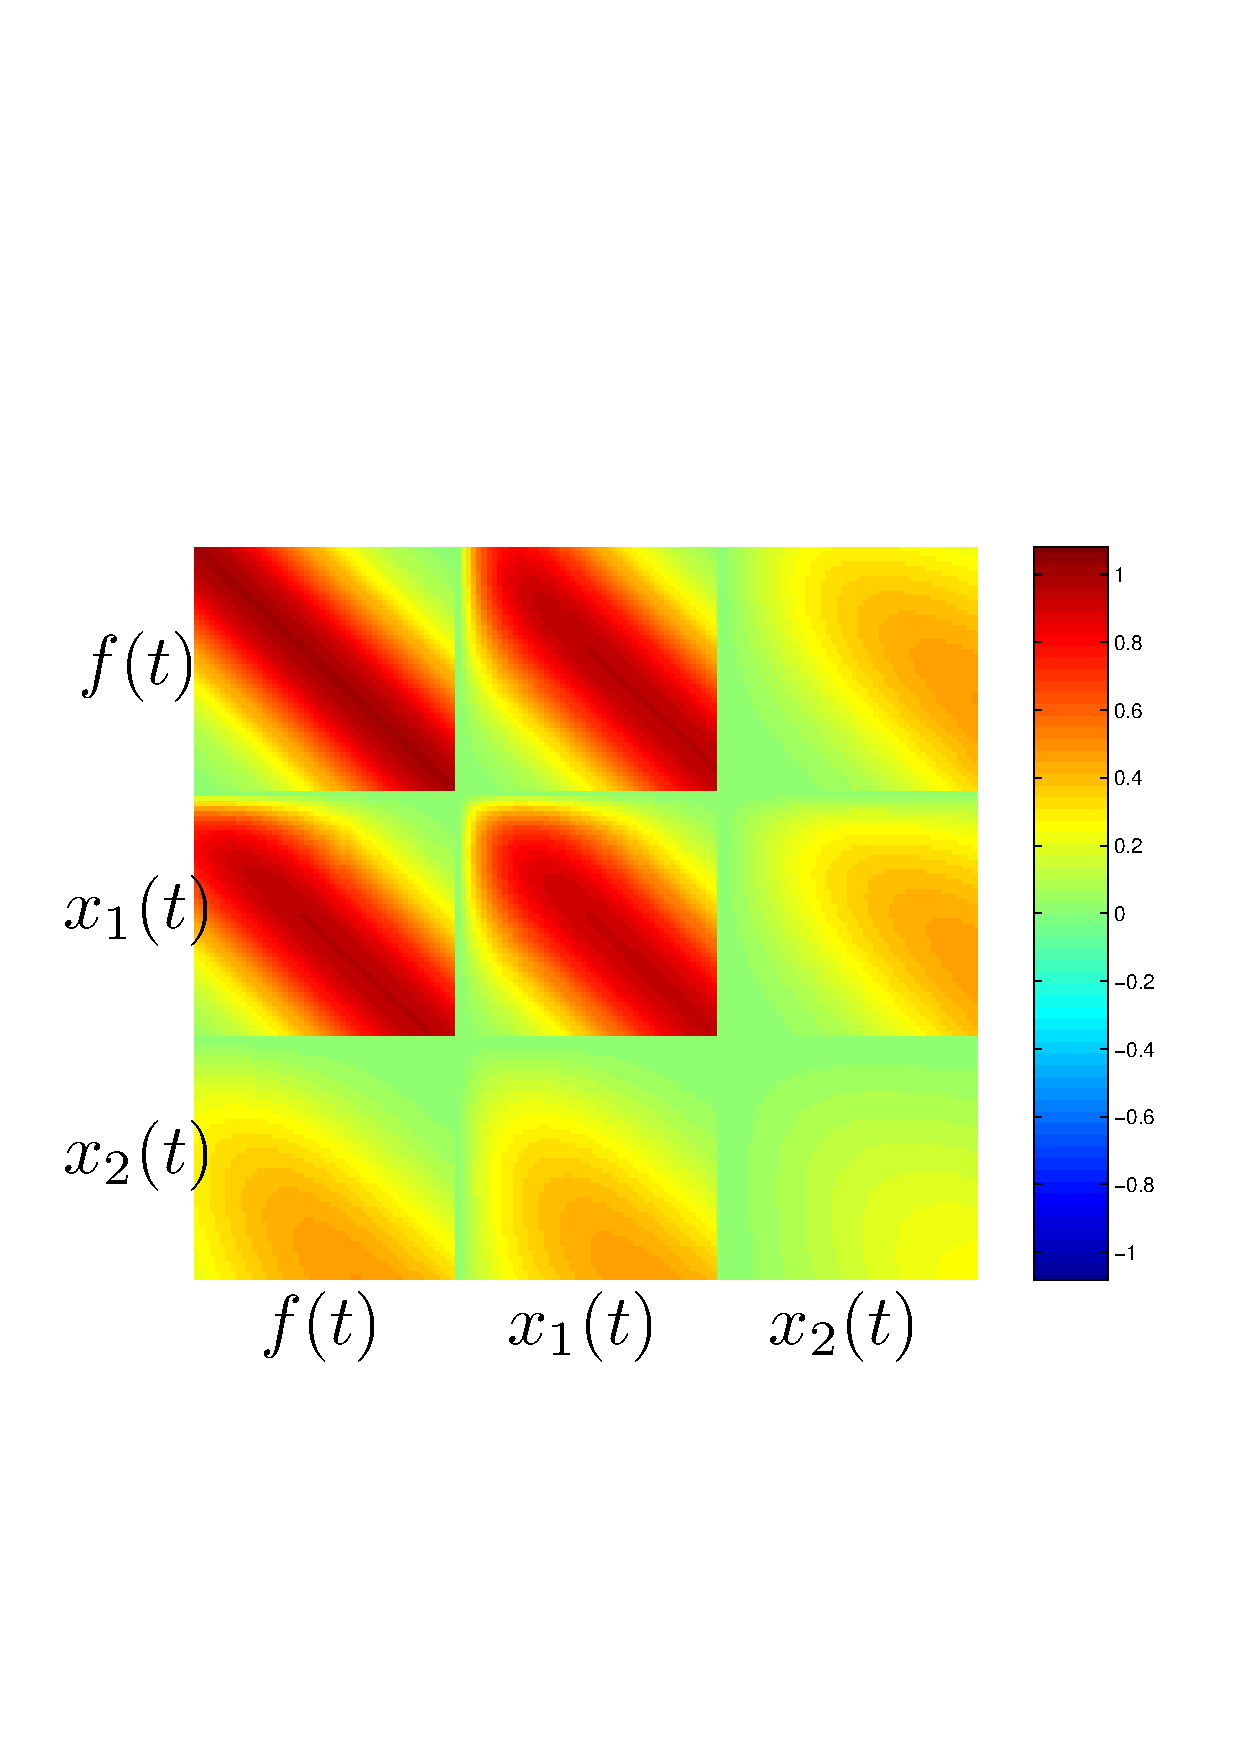
\includegraphics[width=0.8\textwidth]{\lyxdot \lyxdot /diagrams/gpsimTestKernelImage}\par\end{center}%
\end{minipage}%
{\large \par}

\end{columnbox}
\vspace{0.25cm}{\LARGE \par}

\begin{columnbox}


\mysection{Joint Sampling of $x\left(t\right)$ and $f\left(t\right)$ }

\medskip{}
%
\begin{minipage}[c][1\totalheight]{1\columnwidth}%
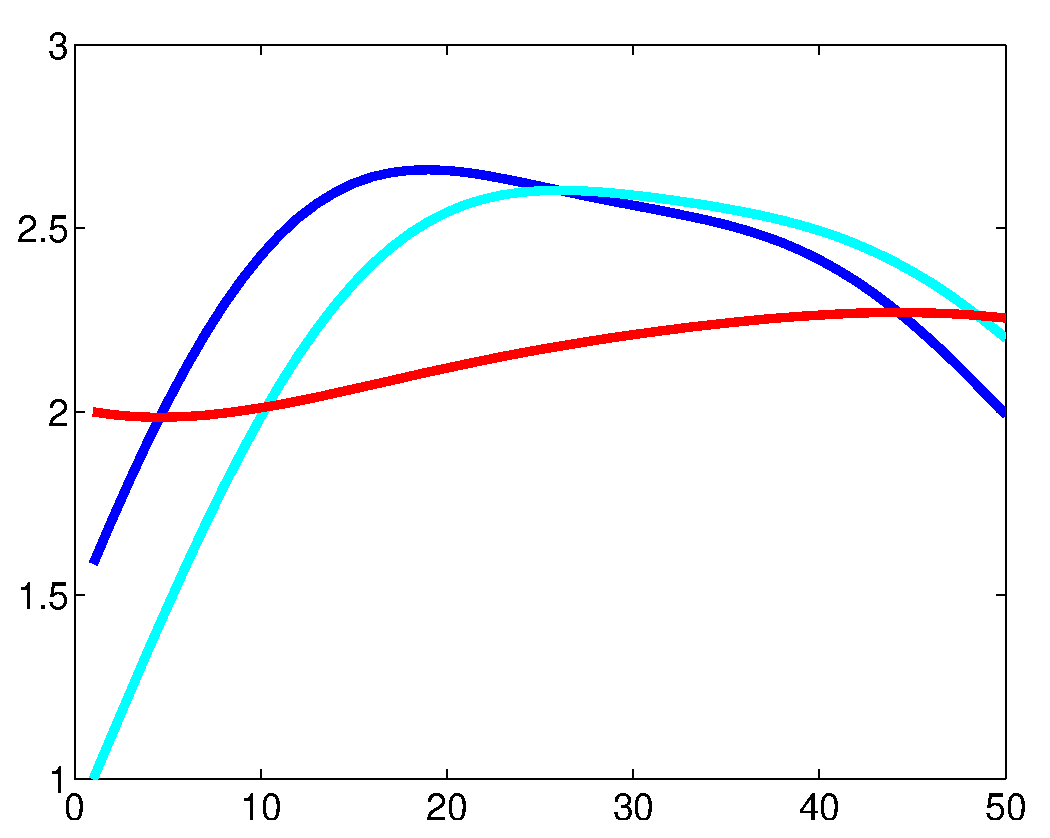
\includegraphics[width=0.4\textwidth]{\lyxdot \lyxdot /\lyxdot \lyxdot /\lyxdot \lyxdot /gp/tex/diagrams/gpsimTestSamples4}\hfill{}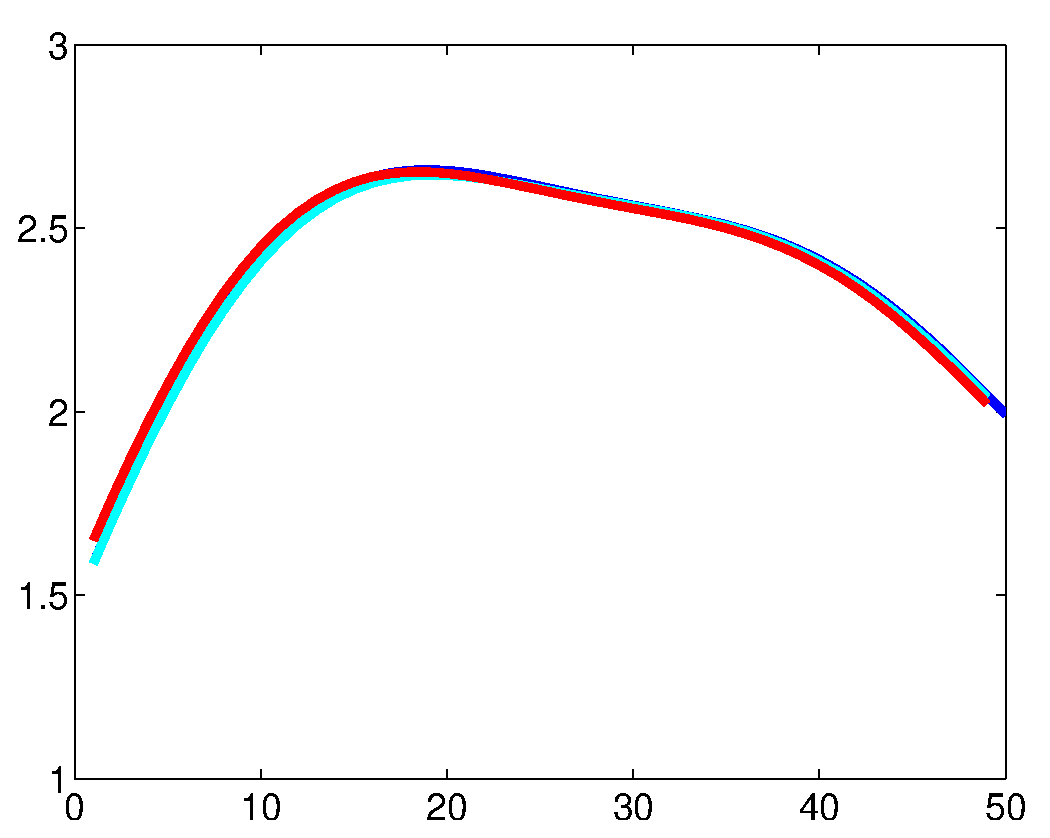
\includegraphics[width=0.4\textwidth]{\lyxdot \lyxdot /\lyxdot \lyxdot /\lyxdot \lyxdot /gp/tex/diagrams/gpsimTestSamples5}\\
{\LARGE \par}

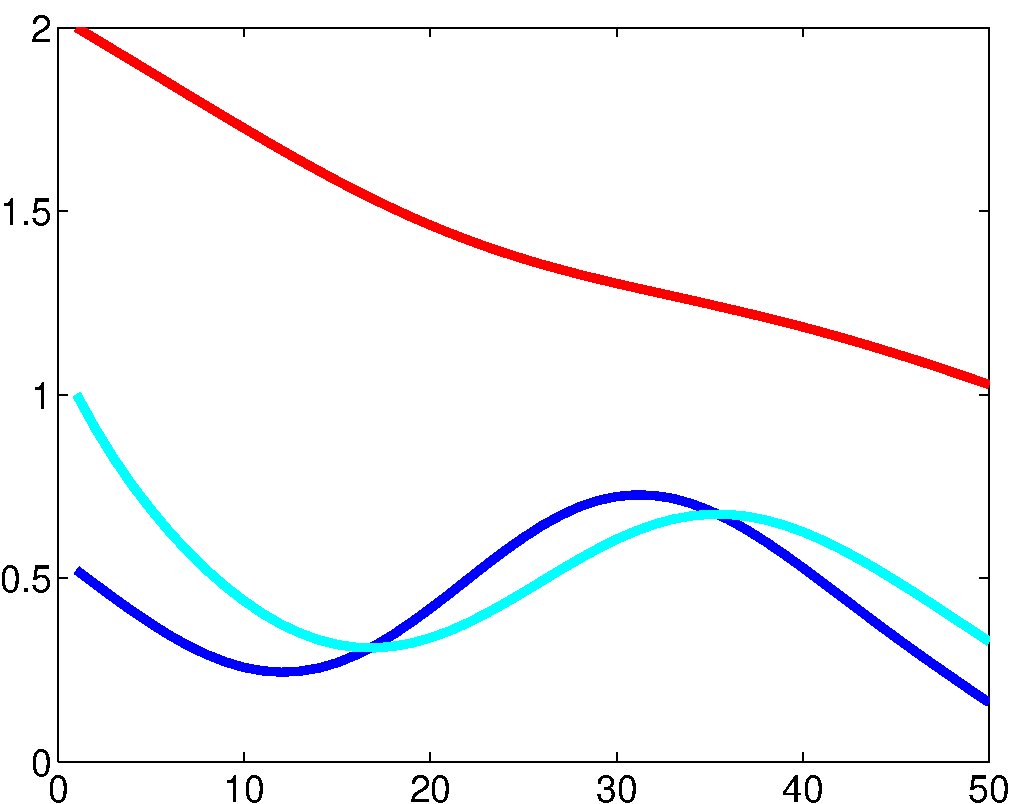
\includegraphics[width=0.4\textwidth]{\lyxdot \lyxdot /\lyxdot \lyxdot /\lyxdot \lyxdot /gp/tex/diagrams/gpsimTestSamples6}\hfill{}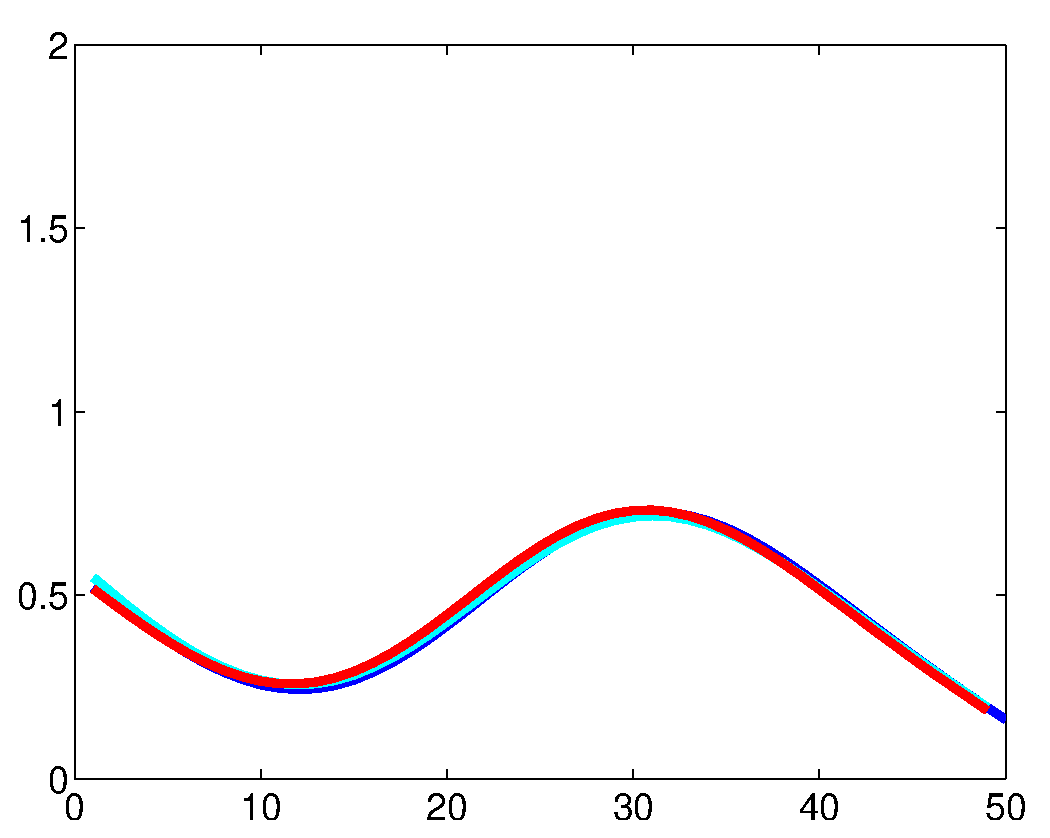
\includegraphics[width=0.4\textwidth]{\lyxdot \lyxdot /\lyxdot \lyxdot /\lyxdot \lyxdot /gp/tex/diagrams/gpsimTestSamples7}\emph{\small }\\
\textrm{\emph{\small Left}}\textrm{\small : joint samples from the
transcription covariance,} \textrm{\emph{\small blue}}\textrm{\small :
$f\left(t\right)$,} \textrm{\emph{\small cyan}}\textrm{\small : $y_{1}\left(t\right)$
and} \textrm{\emph{red}}\textrm{\small : $y_{2}\left(t\right)$.}
\textrm{\emph{\small Right}}\textrm{\small : numerical solution for
$f\left(t\right)$ of the differential equation from $x_{1}\left(t\right)$
and $x_{2}\left(t\right)$ (blue and cyan). True $f\left(t\right)$
included for comparison.} \textrm{\emph{\small }}%
\end{minipage}%
{\large \par}

\end{columnbox}
\vspace{0.25cm}{\LARGE \par}

\begin{columnbox}




\mysection{Covariance Function Computation}

\begin{itemize}
\item We rewrite equation (\ref{solution}) as\[
x_{j}\left(t\right)=\frac{B_{j}}{D_{j}}+L_{j}\left[f\right]\left(t\right)\]
 where \begin{equation}
L_{j}\left[f\right]\left(t\right)=S_{j}\exp\left(-D_{j}t\right)\int_{0}^{t}f\left(u\right)\exp\left(D_{j}u\right)du\label{operators}\end{equation}
 is a linear operator.{\large \par}
\item The new covariance function is then given by\[
\textrm{cov}\left(L_{j}\left[f\right]\left(t\right),L_{k}\left[f\right]\left(t^{\prime}\right)\right)=L_{j}\otimes L_{k}\left[k_{ff}\right]\left(t,t^{\prime}\right).\]
more explicitly {\footnotesize \begin{equation}
k_{x_{j}x_{k}}\left(t,t^{\prime}\right)=S_{j}S_{k}\exp\left(-D_{j}t-D_{k}t^{\prime}\right)\int_{0}^{t}\exp\left(D_{j}u\right)\int_{0}^{t^{\prime}}\exp\left(D_{k}u^{\prime}\right)k_{ff}\left(u,u^{\prime}\right)du^{\prime}du.\label{margCov}\end{equation}
}{\footnotesize \par}
\item For an RBF covariance for $f\left(t\right)$ \[
k_{ff}\left(t,t^{\prime}\right)=\exp\left(-\frac{\left(t-t^{\prime}\right)^{2}}{l^{2}}\right),\]
 these integrals are tractable.{\large \par}
\end{itemize}
\end{columnbox}
\vspace{0.25cm}{\LARGE \par}

\begin{columnbox}


\mysection{Noise Corruption}

\begin{itemize}
\item Allow the mRNA abundance of each gene at each time point to be corrupted
by noise, for observations at $t_{i}$ for $i=1,\ldots,T$ , \begin{equation}
y_{j}\left(t_{i}\right)=x_{j}\left(t_{i}\right)+\epsilon_{j}\left(t_{i}\right)\label{noisyData}\end{equation}
 with $\epsilon_{j}\left(t_{i}\right)\sim\mathcal{N}\left(0,\sigma_{ji}^{2}\right)$. {\large \par}
\item Estimate noise level using probe-level processing techniques of Affymetrix
microarrays (\emph{e.g.} mmgMOS, \citet{Liu:mmgMOS05}). {\large \par}
\item The covariance of the noisy process is then $K_{\mathbf{y}\mathbf{y}}=\Sigma+K_{\mathbf{x}\mathbf{x}}$,
with $\Sigma=\textrm{diag}\left(\sigma_{11}^{2},\ldots,\sigma_{1T}^{2},\ldots,\sigma_{N1}^{2},\ldots,\sigma_{NT}^{2}\right)$.{\large \par}
\end{itemize}
\end{columnbox}
\vspace{0.25cm}{\LARGE \par}

\begin{columnbox}


\mysection{Artificial Data}

\begin{itemize}
\item Results from an artificial data set. {\large \par}

\begin{itemize}
\item We used a `known TFC' and derived six `mRNA profiles'. {\large \par}
\item Fourteen subsamples were taken and corrupted by noise. {\large \par}
\item This `data' was then used to infer a distribution over plausible TFCs.{\large \par}
\end{itemize}
\end{itemize}
\end{columnbox}
\vspace{0.25cm}{\LARGE \par}

\begin{columnbox}


\mysection{Artificial Data Results}

\medskip{}
%
\begin{minipage}[c][1\totalheight]{1\columnwidth}%
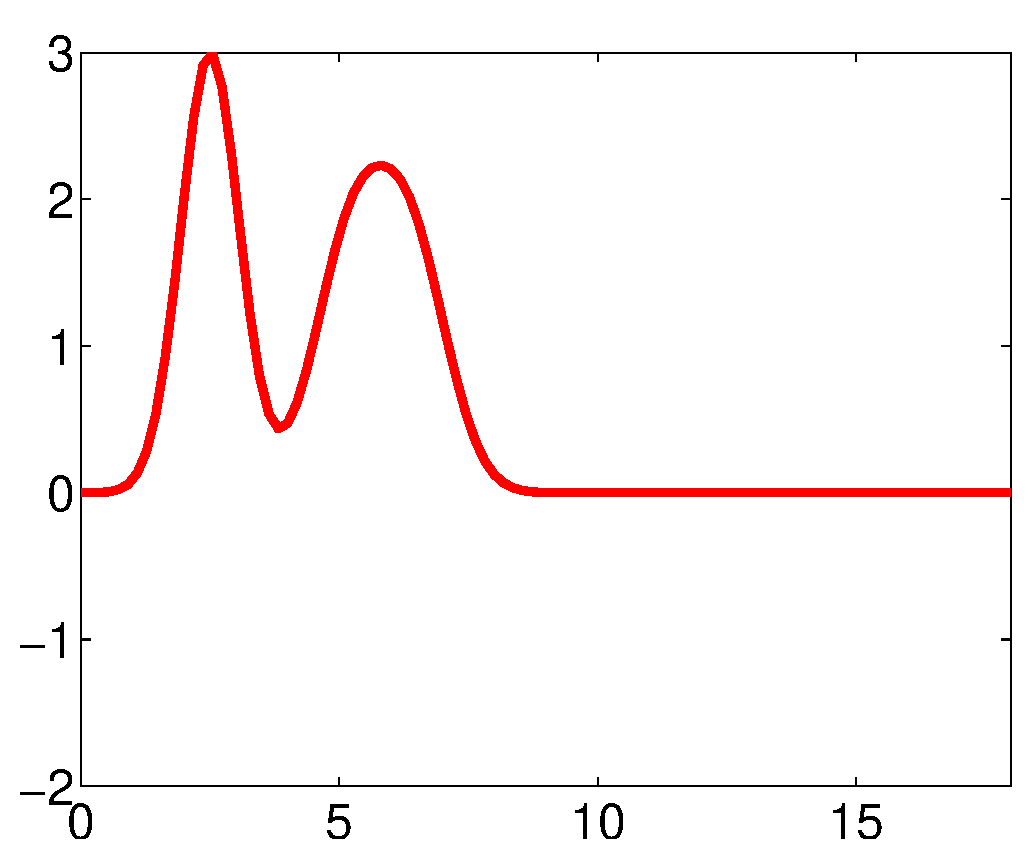
\includegraphics[width=0.3\textwidth]{\lyxdot \lyxdot /\lyxdot \lyxdot /\lyxdot \lyxdot /proposals/gpsimEPSRC/demToyProblem1_true}\hfill{}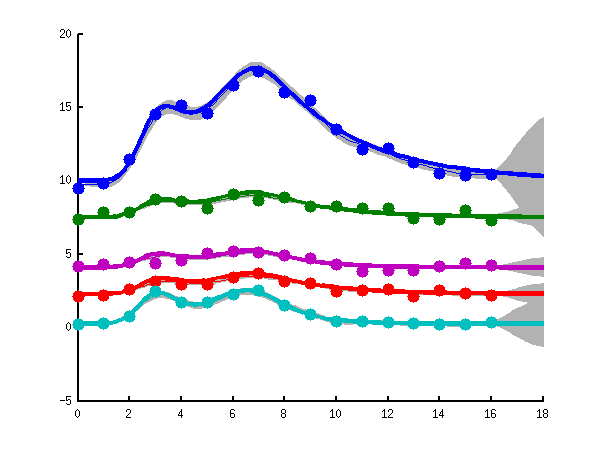
\includegraphics[width=0.3\textwidth]{\lyxdot \lyxdot /\lyxdot \lyxdot /\lyxdot \lyxdot /proposals/gpsimEPSRC/demToyProblem1_genes}\hfill{}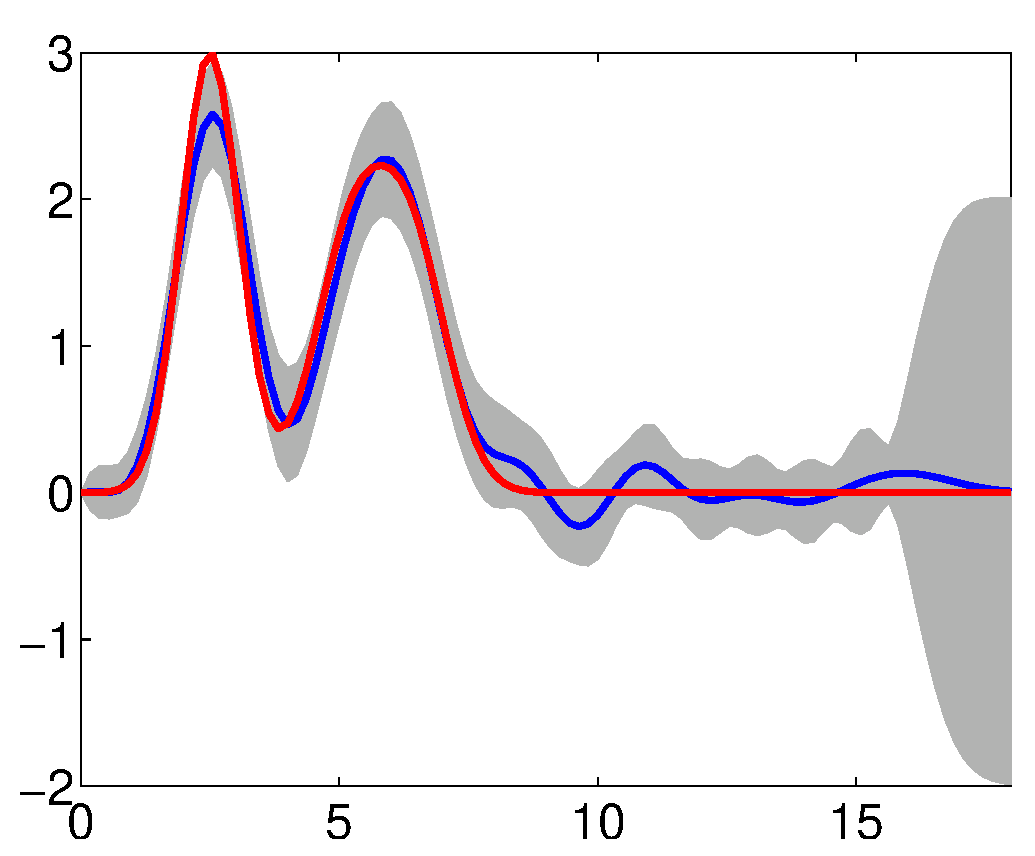
\includegraphics[width=0.3\textwidth]{\lyxdot \lyxdot /\lyxdot \lyxdot /\lyxdot \lyxdot /proposals/gpsimEPSRC/demToyProblem1_infered}{\LARGE \par}

{\footnotesize In this figure we illustrate inference of TFC from
an artificial data set.} \emph{\footnotesize Left:} {\footnotesize The
TFC, $f\left(t\right)$, which drives the system, it is given by the
sum of three Gaussian basis functions.} \emph{\footnotesize Middle:}
{\footnotesize Six gene mRNA concentration profiles each obtained
by using different parameter sets $\left\{ B_{i},S_{i},D_{i}\right\} _{i=1}^{6}$
(lines) along with noise corrupted `data' for the system (crosses).}
\emph{\footnotesize Right:} {\footnotesize The inferred TFC (with
error bars). We used our Gaussian process framework to learn the system's
parameters and infer the TFC.\label{fig:artificialData}}%
\end{minipage}%
{\large \par}

\end{columnbox}
\vspace{0.25cm}{\LARGE \par}

\begin{columnbox}


\mysection{Non-linear Response Model}

\label{sec:nonlinear}{\large \par}

\begin{itemize}
\item Linear model does not account for saturation.{\large \par}
\item All the quantities in equation (\ref{eq:diffEqn}) are positive, but
direct samples from a GP will not be.{\large \par}
\item \emph{Solution}: model response using a positive nonlinear function. {\large \par}
\end{itemize}
\end{columnbox}
\vspace{0.25cm}{\LARGE \par}

\begin{columnbox}


\mysection{Formalism}

\begin{itemize}
\item Introduce a non-linearity $g\left(\cdot\right)$ parameterised by
$\boldsymbol{\theta}_{j}$ \begin{equation}
\begin{split} & \frac{dx_{j}}{dt}=B_{j}+g(f(t),\boldsymbol{\theta}_{j})-D_{j}x_{j}\\
 & x_{j}(t)=\frac{B_{j}}{D_{j}}+\textrm{exp}\left(-D_{j}t\right)\int_{0}^{t}\mathrm{d}u\, g(f(u),\boldsymbol{\theta}_{j})\,\textrm{exp}\left(D_{j}u\right)\ ..\end{split}
\end{equation}
 {\large \par}
\item The induced distribution of $x_{j}(t)$ is no longer a GP.{\large \par}
\item Derive the functional gradient and learn a MAP solution for $f(t)$.{\large \par}
\item Also compute Hessian so we can approximate the marginal likelihood.{\large \par}
\end{itemize}
\end{columnbox}
\vspace{0.25cm}{\LARGE \par}

\begin{columnbox}


\mysection{Log Likelihood}

\begin{itemize}
\item Given noise-corrupted data $y_{j}\left(t_{i}\right)$ the log-likelihood
is {\scriptsize \begin{equation}
\log p(Y|f,\{ B_{j},\theta_{j},D_{j},\Xi\})=-\frac{1}{2}\sum_{i=1}^{T}\sum_{j=1}^{N}\left[\frac{\left(x_{j}(t_{i})-y_{j}\left(t_{i}\right)\right)^{2}}{\sigma_{ji}^{2}}-\log\left(\sigma_{ji}^{2}\right)\right]-\frac{NT}{2}\log(2\pi)\end{equation}
}{\scriptsize \par}


\begin{center}$\Xi$ --- kernel parameters.\par\end{center}{\large \par}

\item The functional derivative of the log-likelihood wrt $f$ is \begin{equation}
\frac{\delta\log p(Y|f)}{\delta f\left(t\right)}=-\sum_{i=1}^{T}\Theta(t_{i}-t)\sum_{j=1}^{N}\frac{(x_{j}(t_{i})-y_{j}\left(t_{i}\right))}{\sigma_{ji}^{2}}g'(f(t))\mathrm{e}^{-D_{j}(t_{i}-t)}\end{equation}
{\large \par}


\begin{center}$\Theta(x)$ --- Heaviside step function. \par\end{center}{\large \par}

\item The negative Hessian of the log-likelihood wrt $f$ is {\scriptsize \begin{equation}
\begin{split}w(t,t^{\prime})= & -\frac{\delta^{2}\log p(Y|f)}{\delta f\left(t\right)\delta f\left(t^{\prime}\right)}=\sum_{i=1}^{T}\Theta(t_{i}-t)\delta\left(t-t^{\prime}\right)\sum_{j=1}^{N}\frac{\left(x_{j}(t_{i})-y_{j}\left(t_{i}\right)\right)}{\sigma_{ji}^{2}}g''(f(t))\mathrm{e}^{-D_{j}(t_{i}-t)}\\
 & +\sum_{i=1}^{T}\Theta(t_{i}-t)\Theta\left(t_{i}-t^{\prime}\right)\sum_{j=1}^{N}\sigma_{ji}^{-2}g'\left(f(t)\right)g'\left(f(t^{\prime})\right)\mathrm{e}^{-D_{j}(2t_{i}-t-t^{\prime})}\end{split}
\end{equation}
}{\scriptsize \par}


\begin{center}$g'(f)=\partial g/\partial f$ and $g^{\prime\prime}(f)=\partial^{2}g/\partial f^{2}$. \par\end{center}{\large \par}

\end{itemize}
\end{columnbox}
\vspace{0.25cm}{\LARGE \par}

\begin{columnbox}


\mysection{Implementation}

\begin{itemize}
\item Implementation requires a discretised time.{\large \par}
\item Compute the gradient and Hessian on a grid.{\large \par}
\item Integrate them by approximate Riemann quadrature.{\large \par}
\item We choose a uniform grid $\left\{ t_{p}\right\} _{p=1}^{M}$ so that
$\Delta=t_{p}-t_{p-1}$ is constant. {\large \par}
\item The vector $\mathbf{f}=\left\{ f_{p}\right\} _{p=1}^{M}$ is the function
$f$ at the grid points. {\large \par}
\item The gradient of the log-likelihood is then given by, {\footnotesize \begin{equation}
\frac{\partial\log p(Y|\mathbf{f})}{\partial f_{p}}=-\Delta\sum_{i=1}^{T}\Theta\left(t_{i}-t_{p}\right)\sum_{j=1}^{N}\frac{\left(x_{j}\left(t_{i}\right)-y_{j}\left(t_{i}\right)\right)}{\sigma_{ji}^{2}}g'\left(f_{p}\right)\mathrm{e}^{-D_{j}\left(t_{i}-t_{p}\right)}\label{funcGrad}\end{equation}
} {\large \par}
\item Negative Hessian of the log-likelihood is, {\scriptsize \begin{equation}
\begin{split} & W_{pq}=-\frac{\partial^{2}\log p(Y|\mathbf{f})}{\partial f_{p}\partial f_{q}}=\delta_{pq}\Delta\sum_{i=1}^{T}\Theta\left(t_{i}-t_{q}\right)\sum_{j=1}^{N}\frac{\left(x_{j}\left(t_{i}\right)-y_{j}\left(t_{i}\right)\right)}{\sigma_{ji}^{2}}g''\left(f_{q}\right)\mathrm{e}^{-D_{j}\left(t_{i}-t_{q}\right)}\\
 & +\:\Delta^{2}\sum_{i=1}^{T}\Theta\left(t_{i}-t_{p}\right)\Theta\left(t_{i}-t_{q}\right)\sum_{j=1}^{N}\sigma_{ji}^{-2}g'\left(f_{q}\right)g'\left(f_{p}\right)\mathrm{e}^{-D_{j}\left(2t_{i}-t_{p}-t_{q}\right)}\end{split}
\label{funcHess}\end{equation}
} where $\delta_{pq}$ is the Kronecker delta. {\large \par}
\end{itemize}
\end{columnbox}
\vspace{0.25cm}{\LARGE \par}

\begin{columnbox}


\mysection{Implementation II}

\begin{itemize}
\item Combine these with prior to compute gradient and Hessian of log posterior
$\Psi(\mathbf{f})=\log p(Y|\mathbf{f})+\log p(\mathbf{f})$ \citep[see][chapter 3]{Rasmussen:book05}
\begin{equation}
\begin{split} & \frac{\partial\Psi(\mathbf{f})}{\partial\mathbf{f}}=\frac{\partial\log p(Y|\mathbf{f})}{\partial\mathbf{f}}-K^{-1}{\mathbf{f}}\\
 & \frac{\partial^{2}\Psi(\mathbf{f})}{\partial\mathbf{f}^{2}}=-(W+K^{-1})\end{split}
\label{postGrid}\end{equation}
 $K$ prior covariance evaluated at the grid points. {\large \par}
\item Use to find a MAP solution via, $\hat{\mathbf{f}}$, using Newton's
algorithm. {\large \par}
\item The Laplace approximation is then \begin{equation}
\log p(Y)\simeq\log p(Y|\hat{\mathbf{f}})-\mbox{$\frac{1}{2}$}\hat{\mathbf{f}}^{T}K^{-1}\hat{\mathbf{f}}-\mbox{$\frac{1}{2}$}\log|I+KW|.\label{eqn_marginal}\end{equation}
 {\large \par}
\end{itemize}
\end{columnbox}
\vspace{0.25cm}{\LARGE \par}

\begin{columnbox}


\mysection{Example: exponential response}

\begin{itemize}
\item Exponential response constrains protein concentration positive. \begin{equation}
g\left(f\left(t\right),\theta_{j}\right)=S_{j}\textrm{exp}\left(f\left(t\right)\right)\label{expResp}\end{equation}
{\large \par}
\end{itemize}
\end{columnbox}
\vspace{0.25cm}{\LARGE \par}

\begin{columnbox}


\mysection{Results}

\begin{itemize}
\item Recently published biological data set studied using linear response
model by \citet{Barenco:ranked06}. {\large \par}
\item Study focused on the tumour suppressor protein p53. {\large \par}
\item mRNA abundance measured at regular intervals using Affymetrix U133A
oligonucleotide microarrays. {\large \par}
\item Five known target genes of p53: \emph{DDB2}, \emph{p21}, \emph{SESN1/hPA26},
\emph{BIK} and \emph{TNFRSF10b}. {\large \par}
\item They used quadratic interpolation for  the mRNA production rates,
discretised the model, and used MCMC sampling to obtain estimates
of the model parameters $B_{j}$, $S_{j}$, $D_{j}$ and $f(t)$. {\large \par}
\item Sensitivity and mRNA decay of one target gene, p21, was fixed and
$f(0)$ was constrained to be zero. {\large \par}
\end{itemize}
\end{columnbox}
\vspace{0.25cm}{\LARGE \par}

\begin{columnbox}


\mysection{Linear response analysis}

\begin{itemize}
\item We analysed data using the linear response model{\large \par}
\item Raw data was processed using the mmgMOS model of \citet{Liu:mmgMOS05}
which provides variance as well as expression level.{\large \par}
\item Inferred posterior mean function shown below for RBF kernels.{\large \par}
\item Note oscillatory behaviour, possible artifact of RBF covariance \citep[see page 123 in][]{Rasmussen:book05}. {\large \par}
\item We repeated the experiment using the {}``MLP'' covariance function
\citet{Williams:computation98}. \begin{equation}
\begin{split}k\left(t,t'\right)=\textrm{arcsin}\left(\frac{wtt'+b}{\sqrt{\left(wt^{2}+b+1\right)\left(wt'^{2}+b+1\right)}}\right)\end{split}
\end{equation}
{\large \par}
\end{itemize}
\end{columnbox}
\vspace{0.25cm}{\LARGE \par}

\begin{columnbox}


\mysection{Linear Response Results}

\medskip{}
%
\begin{minipage}[c][1\totalheight][t]{1\columnwidth}%
\begin{center}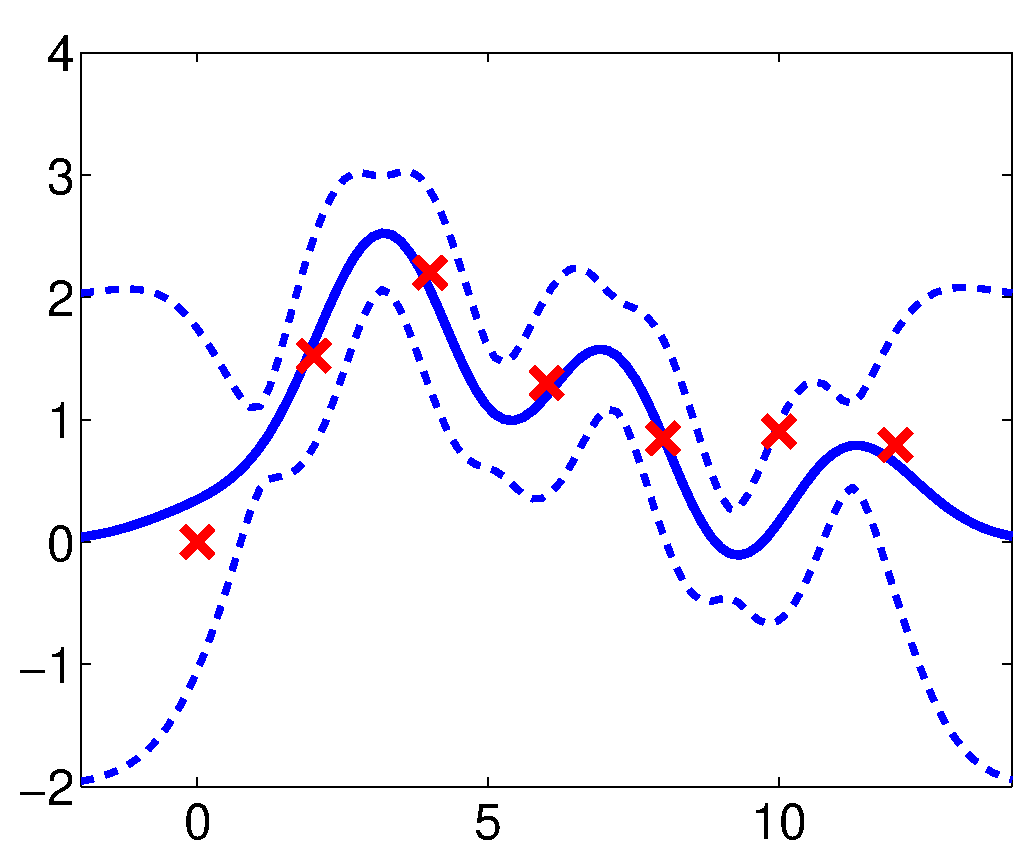
\includegraphics[width=0.45\textwidth]{\lyxdot \lyxdot /diagrams/demBarenco1_profile1_slides}\hfill{}\includegraphics[width=0.45\textwidth]{\lyxdot \lyxdot /diagrams/demBarencoMap2MlpLin_profile1_slide} \par\end{center}{\LARGE \par}

\textrm{\small Predicted protein concentration for p53 using a linear
response model:} \textrm{\emph{\small Left:}} \textrm{\small RBF prior
on $f$;} \textrm{\emph{\small Right:}} \textrm{\small MLP prior on
$f$. Solid line is mean prediction, dashed lines are 95\% credibility
intervals. The prediction of Barenco} \textrm{\emph{\small et al.}}
\textrm{\small was pointwise and is shown as crosses.}{\small \par}

\textrm{\small \label{cap:barencoComparisonProfile} }%
\end{minipage}%
{\large \par}

\end{columnbox}
\vspace{0.25cm}{\LARGE \par}

\begin{columnbox}


\mysection{Linear Response Results II}

\medskip{}
%
\begin{minipage}[c][1\totalheight][t]{1\columnwidth}%
 {\LARGE \par}

\begin{center}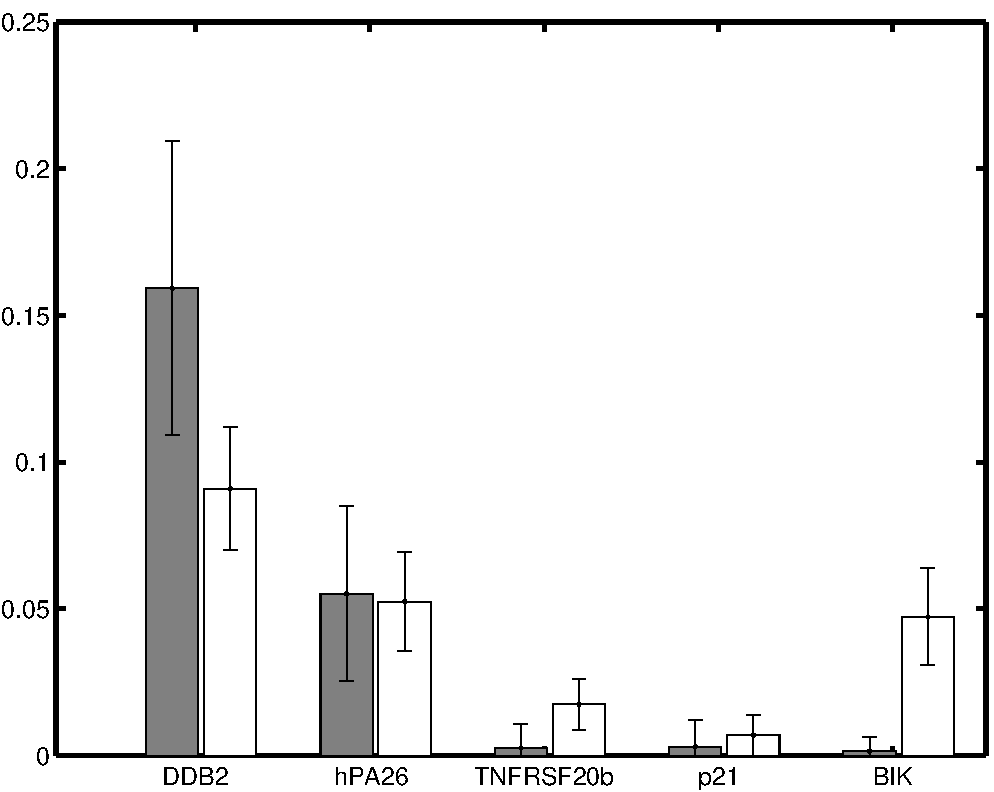
\includegraphics[width=0.3\textwidth]{\lyxdot \lyxdot /diagrams/HMCBaseErrBars}\hfill{}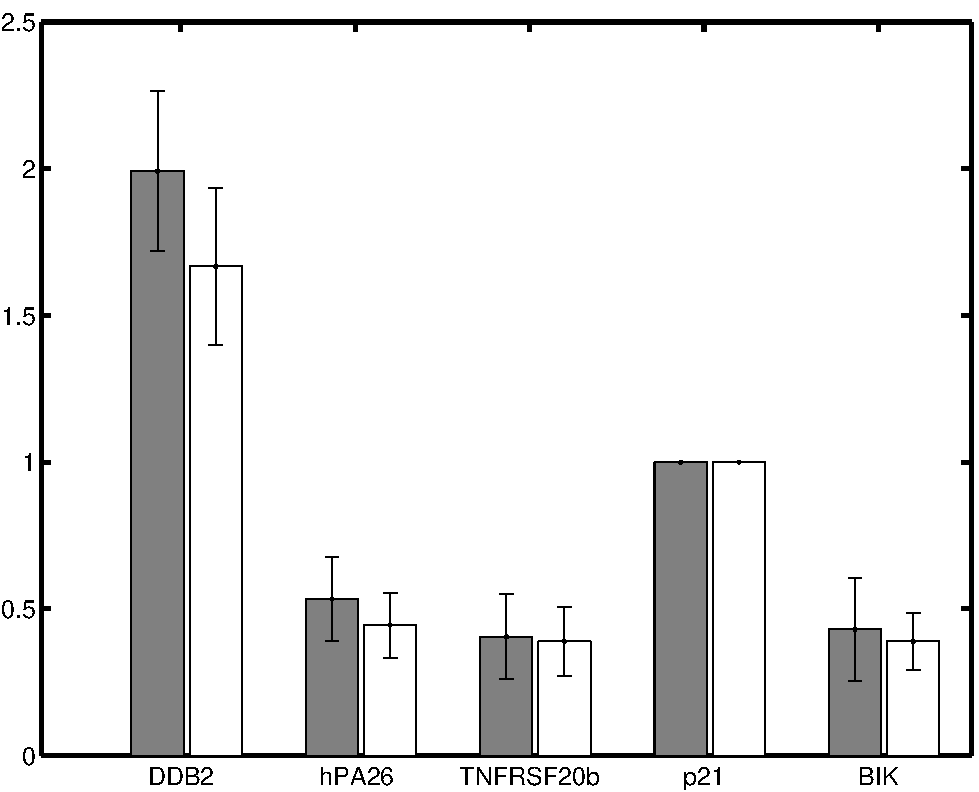
\includegraphics[width=0.3\textwidth]{\lyxdot \lyxdot /diagrams/HMCSensErrBars}\hfill{}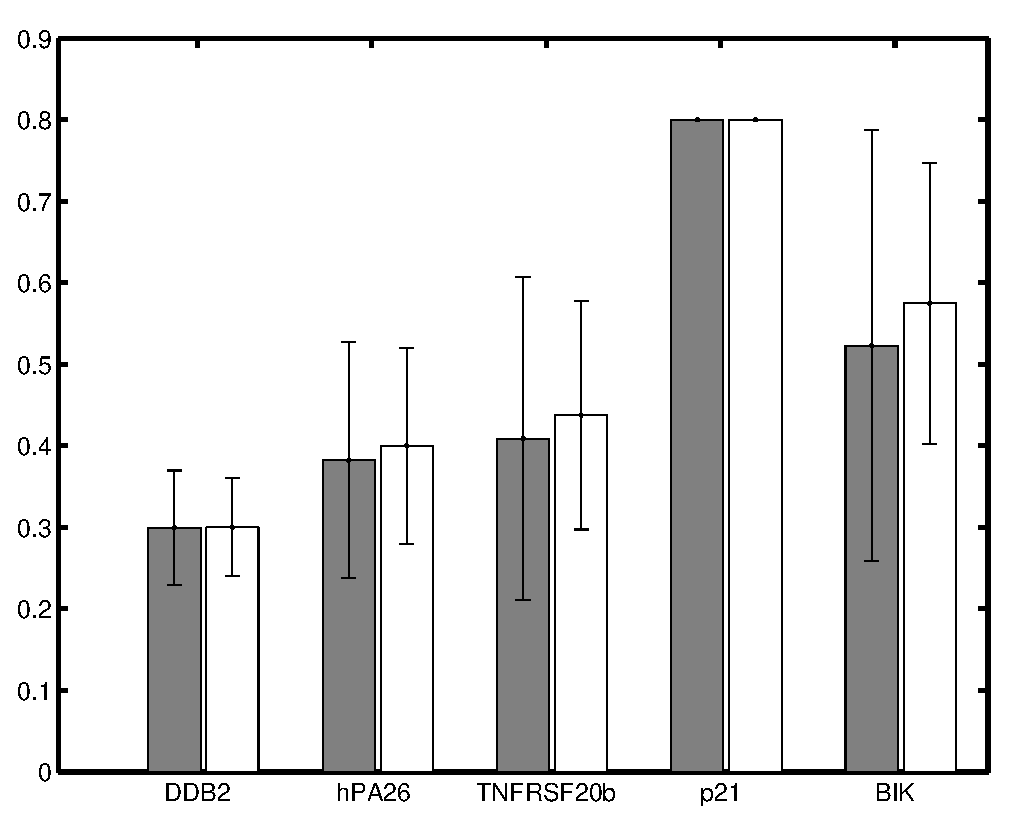
\includegraphics[width=0.3\textwidth]{\lyxdot \lyxdot /diagrams/HMCDecayErrBars}\par\end{center}{\LARGE \par}

\textrm{\small Results of inference on the hyperparameters for p53
data studied in \citet{Barenco:ranked06}. The bar charts show} \textrm{\emph{\small Left:}}
\textrm{\small Basal transcription rates from our model and that of
Barenco} \textrm{\emph{\small et al.}}\textrm{\small . Grey are estimates
obtained with our model, white are the estimates obtained by Barenco}
\textrm{\emph{\small et al.}} \textrm{\small }\textrm{\emph{\small Middle:}}
\textrm{\small Similar for sensitivities.} \textrm{\emph{\small Right:}}
\textrm{\small Similar for decay rates.\label{cap:barencoComparisonBar}}%
\end{minipage}%
{\large \par}

\end{columnbox}
\vspace{0.25cm}{\LARGE \par}

\begin{columnbox}


\mysection{Linear Response Discussion}

\begin{itemize}
\item Figure above shows the results of inference on the values of the hyperparameters
$B_{j}$, $S_{j}$ and $D_{j}$. {\large \par}
\item Samples from the posterior distribution were obtained using Hybrid
Monte Carlo (see \emph{e.g.}~\citealp{Neal:book96}). {\large \par}
\item Results are in good accordance with the results obtained by Barenco
\emph{et al.} {\large \par}
\item Differences in estimates of the basal transcription rates probably
due to the different methods used for probe-level processing of the
microarray data. {\large \par}
\end{itemize}
\end{columnbox}
\vspace{0.25cm}{\LARGE \par}

\begin{columnbox}


\mysection{Non-linear response analysis}

\begin{itemize}
\item Exponential response model (constrains protein concentrations positive). {\large \par}
\item Inferred MAP solutions for the latent function $f$ are plotted below.{\large \par}
\end{itemize}
\end{columnbox}
\vspace{0.25cm}{\LARGE \par}

\begin{columnbox}


\mysection{Non-linear Response Results }

\medskip{}
%
\begin{minipage}[c][1\totalheight][t]{1\columnwidth}%
\begin{center}\includegraphics[width=0.45\textwidth]{\lyxdot \lyxdot /diagrams/demBarencoMap2Rbf_profile1_slide}\hfill{}\includegraphics[width=0.45\textwidth]{\lyxdot \lyxdot /diagrams/demBarencoMap2Mlp_profile1_slide} \par\end{center}{\LARGE \par}

\textrm{\small Predicted protein concentration for p53 using an exponential
response:} \textrm{\emph{\small Left:}} \textrm{\small shows results
of using a squared exponential prior covariance on $f$;} \textrm{\emph{\small Right:}}
\textrm{\small shows results of using an MLP prior covariance on $f$.
Solid line is mean prediction, dashed lines show 95\% credibility
intervals. The results shown are for $\textrm{exp}(f)$, hence the
asymmetry of the credibility intervals. The prediction of Barenco}
\textrm{\emph{\small et al.}} \textrm{\small was pointwise and is
shown as crosses.}{\small \par}

\textrm{\small \label{nonlinearInf}} %
\end{minipage}%
{\large \par}

\end{columnbox}
\vspace{0.25cm}{\LARGE \par}

\begin{columnbox}


\mysection{Discussion}

\begin{itemize}
\item We have described how GPs can be used in modelling dynamics of a simple
regulatory network motif. {\large \par}
\item Our approach has advantages over standard parametric approaches: {\large \par}

\begin{itemize}
\item there is no need to restrict the inference to the observed time points,
the temporal continuity of the inferred functions is accounted for
naturally. {\large \par}
\item GPs allow us to handle uncertainty in a natural way.{\large \par}
\item MCMC parameter estimation in a discretised model can be computationally
expensive. Parameter estimation can be achieved easily in our framework
by type II maximum likelihood or by using efficient hybrid Monte Carlo
sampling techniques {\large \par}
\end{itemize}
\item All code on-line \url{http://www.dcs.shef.ac.uk/~neil/gpsim/}.{\large \par}
\end{itemize}
\end{columnbox}
\vspace{0.25cm}{\LARGE \par}

\begin{columnbox}


\mysection{Future Directions}

\begin{itemize}
\item This is still a very simple modelling situation. {\large \par}

\begin{itemize}
\item We are ignoring transcriptional delays.{\large \par}
\item Should consider more biologically meaningful nonlinearities (\emph{e.g.}
Michaelis-Menten model used in \citet{Rogers:model06b}). {\large \par}
\item Here we have single transcription factor: our ultimate goal is to
describe regulatory pathways with more genes.{\large \par}
\end{itemize}
\item All these issues can be dealt with in the general framework we have
described.{\large \par}

\begin{itemize}
\item Need to overcome the greater computational difficulties.{\large \par}
\end{itemize}
\end{itemize}
\end{columnbox}
\vspace{0.25cm}{\LARGE \par}

\begin{columnbox}


\mysection{Acknowledgements}

\medskip{}
{\scriptsize We thank Martino Barenco for useful discussions and for
providing the data. We gratefully acknowledge support from BBSRC Grant
No BBS/B/0076X {}``Improved processing of microarray data with probabilistic
models''.} {\small } {\scriptsize \bibliographystyle{abbrvnat}
\bibliography{gpip}
}{\scriptsize \par}

\end{columnbox}
\vspace{0.25cm}{\LARGE \par}

\end{multicols}
\end{document}
